\documentclass{article}
\usepackage[utf8]{inputenc}
\usepackage{polski}
\usepackage{graphicx}
\usepackage[margin= 2.5cm]{geometry}
\usepackage{amsmath}
\usepackage{float}
\usepackage[section]{placeins}

\title{Wskaźnik MACD}
\author{Piotr Pesta}
\date{Marzec 2022}
\setlength{\parindent}{20pt}
\graphicspath{{./Graphs/}}

\begin{document}
\maketitle

\section{Wstęp}

    Celem projektu było zaimplementowanie wskaźnika MACD (Moving Average Convergence Divergence), który pozwala na podstawie analizy danych historycznych
    wyznaczać momenty kupna i sprzedaży udziałów. Wskaźnik ten składa się z dwóch krzywych: MACD oraz Signal.
    Implementacji dokonałem w języku Python z wykorzystaniem bibliotek pandas oraz matplotlib.
    Dane wejściowe to plik .csv o zawierający informacje o cenach udziałów z konkretnych dni. 
    Jako wartość udziałów w danym dniu przyjąłem cenę zamknięcia z tego dnia. Do algorytmu obracającego akcjami podajemy dane z ok. 1000 dni.

\section{Analiza zadania}

    W celu określenia na podstawie wskaźnika MACD momentów kupna i sprzedaży akcji należy obliczyć
    dwie średnie kroczące z wartości udziałów:
    \begin{itemize}
        \item krótkookresową - 12 okresów
        \item długookresową - 26 okresów
    \end{itemize}

    \noindent Następnie wartość MACD uzyskujemy odejmując średnią długookresową od krótkookresowej.
    W celu obliczenia Signal należy obliczyć średnią krocząca z MACD z 9 okresów. 


    Do obliczenia średnich kroczących skorzystałem z poniższego wzoru:
 
        

    \begin{align*} 
        EMA_{N} &= \frac{p_{0} + (1-\alpha)p_{1} + (1-\alpha)^2p_{2} + \ldots + (1-\alpha)^Np_{N}}{1 + (1-\alpha)+(1-\alpha)^2 + \ldots + (1-\alpha)^N} \\
        \mathit{Gdzie:} & \\
        \alpha &= \frac{2}{N + 1} \\
        N &- liczba \; okres \mathit{ó} w \\
        p_{i} &- pr\mathit{ó}bka \; z \; i-tego \;dnia, \;p_{0}\; - \; pr\mathit{ó}bka \;z \;aktualnego \;dnia, \;p_{N} \;-\;pr\mathit{ó}bka \;sprzed \;N \;dni.
    \end{align*}

    Punkty, w których krzywa MACD przecina Signal od dołu są sygnałem do kupna akcji oraz zapowiadają trend wzrostowy.
    Natomiast punkty, w których MACD przecina Signal od góry, są sygnałem sprzedaży akcji i zapowiedzią trendu spadkowego. 

\section{Analiza skuteczności i przykłady działania}
    \begin{figure}[H]
        \noindent\makebox[\textwidth]{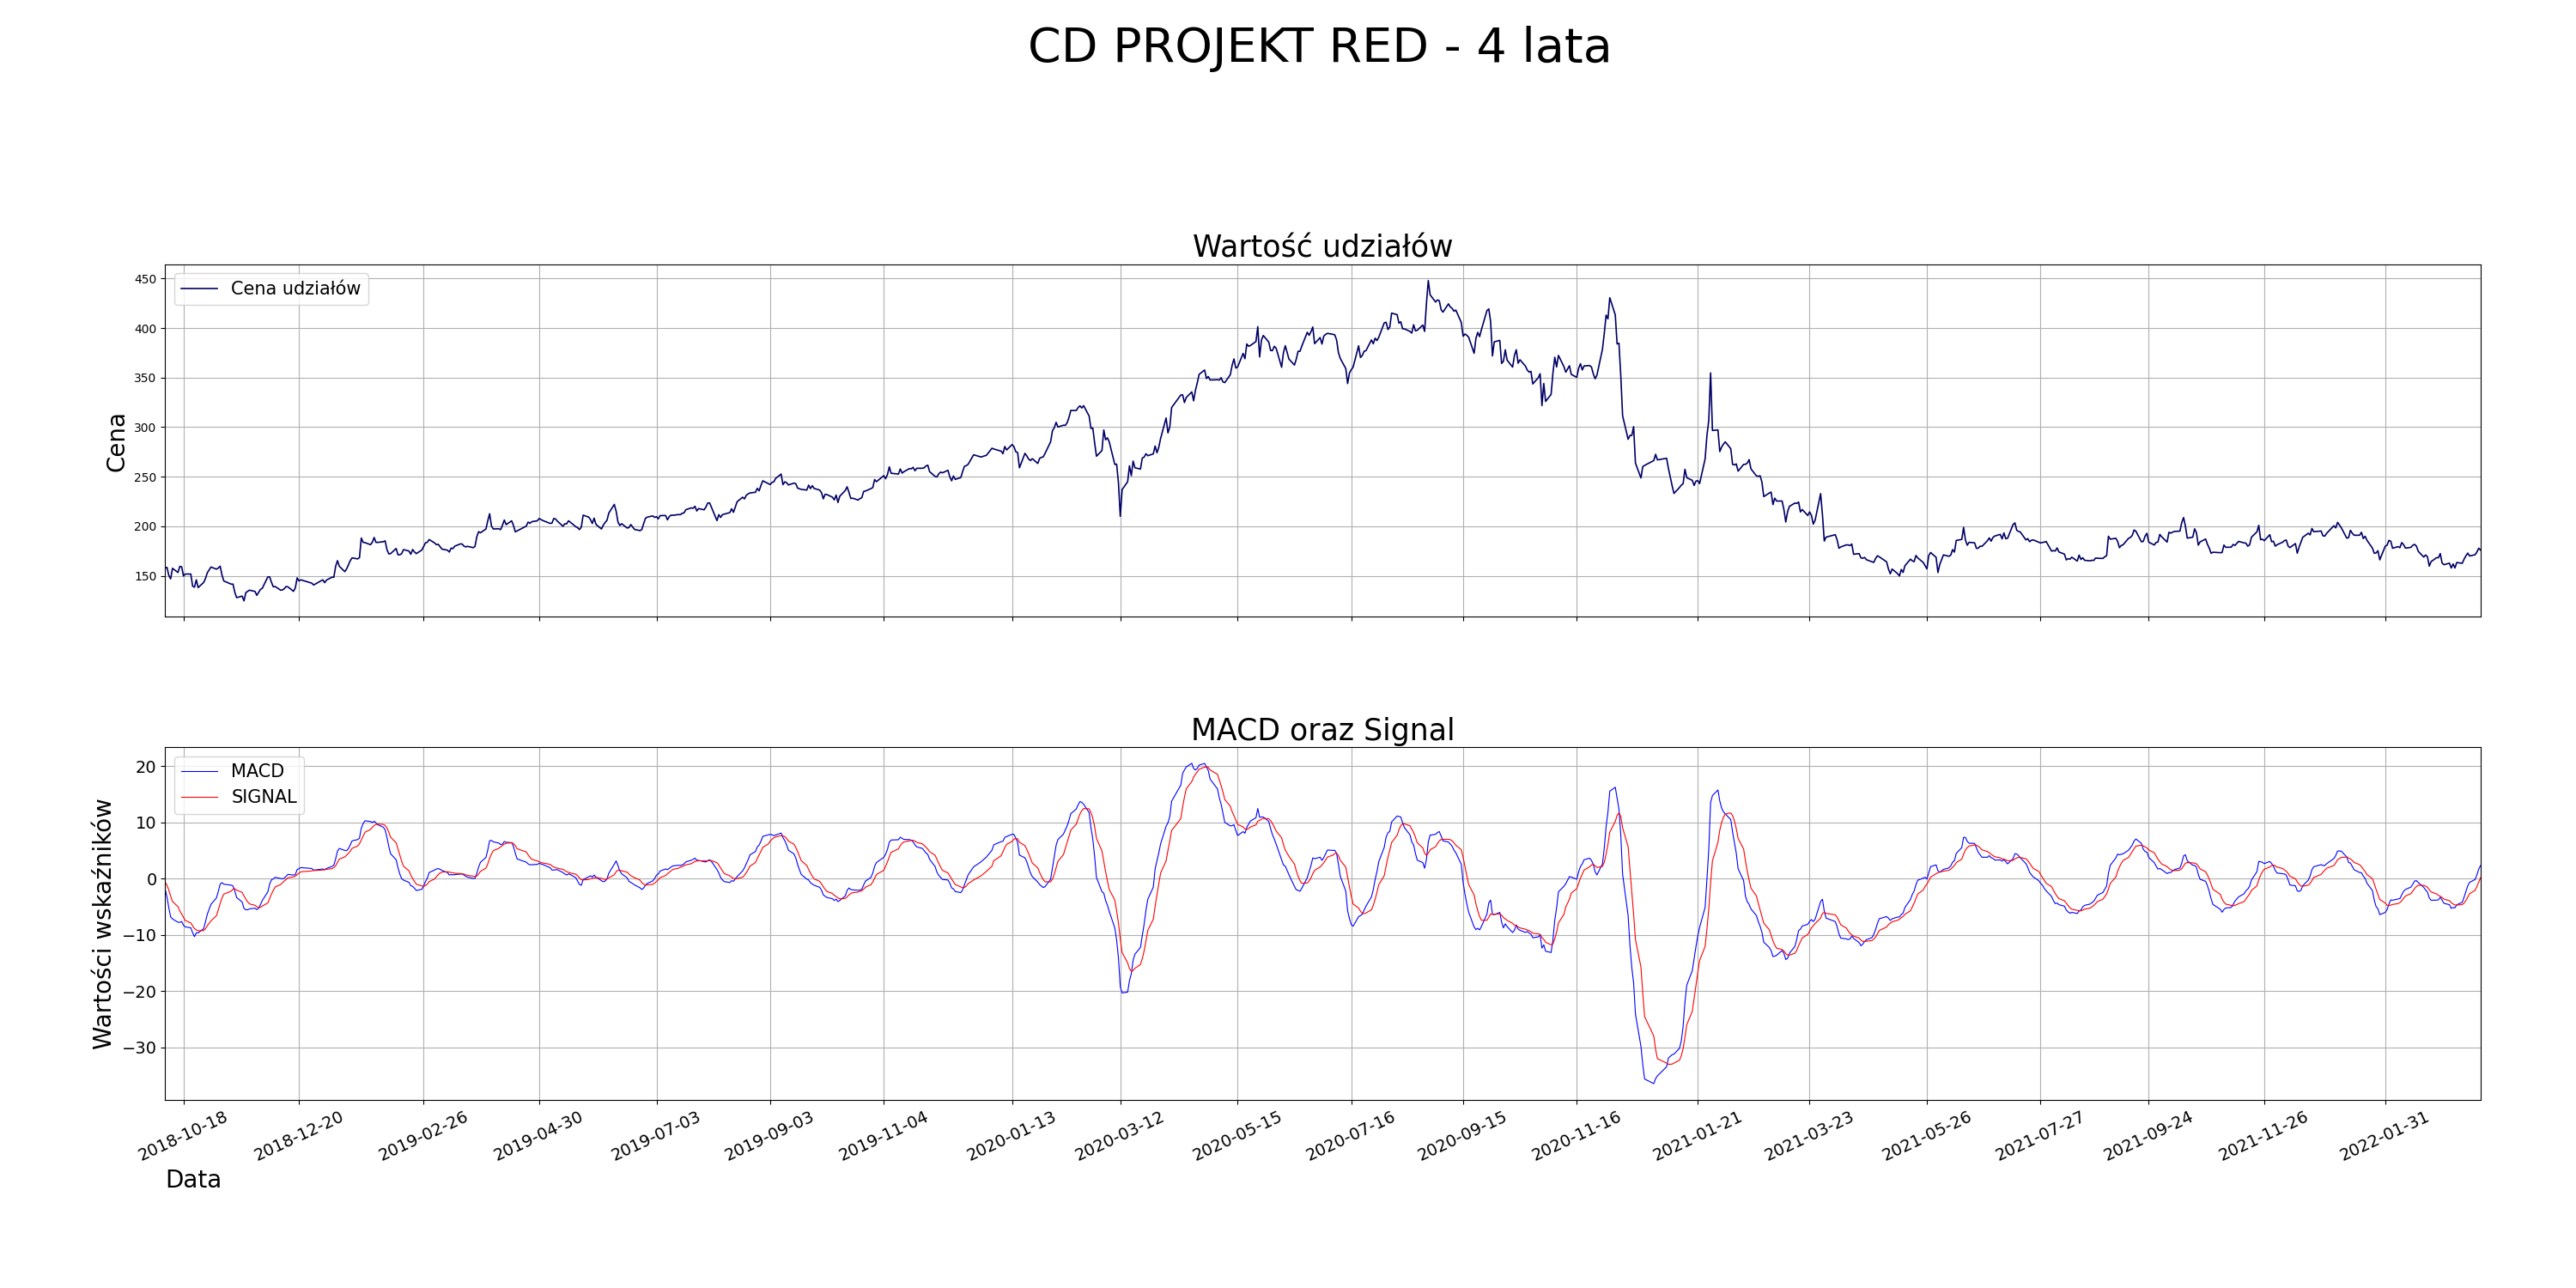
\includegraphics[width=\paperwidth]{CD PROJEKT RED - 4 lata.png}}
        \caption{Wykres ceny udziałów CDR oraz obliczonych na ich podstawie MACD oraz Signal. Wykres ten składa się z ok. 900 cen zamknięcia.
         W celu zachowania czytelności wykresu nie naniosłem na niego linii wyznaczających momenty kupna i sprzedaży.}
    \end{figure}

    Analizując powyższy wykres możemy dojść do kilku wniosków:
    \begin{itemize}
        \item dla powolnych zmian wskaźnik MACD jest skuteczny i pozwala osiągnąć zyski. Jest to dobrze widoczne na wykresie w okresie od 12.03.2022 do 15.05.2020 oraz na lewej części wykresu.
        \item MACD zbyt późno reaguje na nagłe zmiany cen udziałów. Możemy to zauważyć na wykresie w okolicach 21.01.2021, kiedy wystąpił pik wartości udziałów.
         Na pierwszy rzut oka może wydawać się, że wskaźnik zareagował prawidłowo, jednak gdy przyjrzymy się dokładniej to zauważymy, że sygnał sprzedaży jest spóźniony i znajduję się poza pikiem.
         Wskaźnik nie nadążył za zmianą i okazja do niemałego zarobku przepadła.
    \end{itemize}

    \newpage
    Wskaźnik MACD jest przydatny do inwestycji w akcje stabilne, które nie ulegają częstym nagłym zmianom.
    Dla danych przedstawionych na powyższym wykresie prosty algorytm działający jedynie na podstawie MACD
    osiągnął duży zysk - wynik
   
    \begin{figure}[H]
        \noindent\makebox[\textwidth]{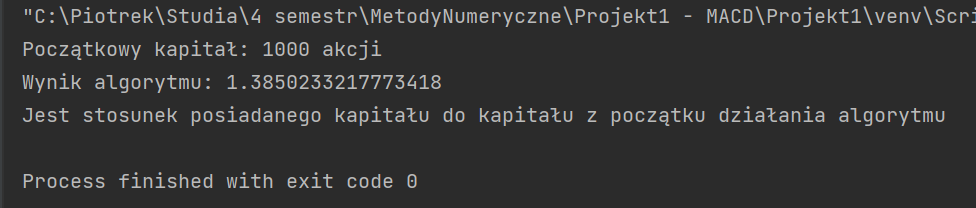
\includegraphics{AnalizaCDP.png}}
        \caption{CDP w latach 2018-2022 - ok. 1.5 krotny zysk}
    \end{figure}
    

\newpage
\section{Analiza przydatności MACD do inwestowania}

    Analziując zachowanie algorytmu dla różnych wejść, możemy zauważyć, że najprostszy algorytm,
    kupujący i sprzedający udziały, nie osiąga zadowalających rezultatów. Dla niekótrych indeksów osiąga
    bardzo dobre wyniki, ale w większości przypadków wartość naszego portfela na końcu testu jest niższa niż na początku.

    
    Efektywność algorytmu określamy jako stosunek wartości naszego portfela
    do jego stanu po działaniu algorytmu na podstawie poniższego wzoru:

    \begin{align*} 
        zysk = \frac{\mathit{ilośćAkcji}(N) \cdot \mathit{cenaAkcji}(N) + \mathit{gotówka}(N)}{1000 \cdot \mathit{cenaAkcji}(0)}
    \end{align*}


    \noindent Wartość poniżej 1 będzie oznaczać stratę, a powyżej zysk.\\
    \noindent Przykładowe wyniki:
    %DO ZMIAN SPORYCH BO BYL ZJEBANY WZOR
    \begin{figure}[H]
        \noindent\makebox[\textwidth]{\includegraphics{AnalizaCDPDługi.png}}
        \caption{CDP w latach 2012-2022 - strata ok. 334 zł}
    \end{figure}
    \begin{figure}[H]
        \noindent\makebox[\textwidth]{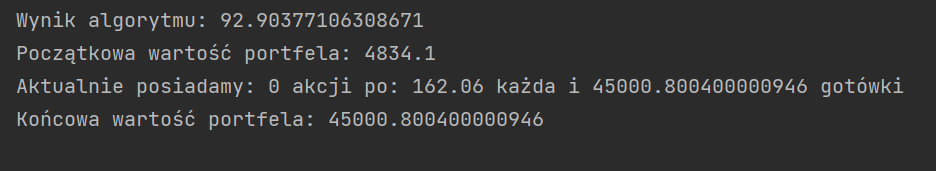
\includegraphics{AnalizaOrlen.png}}
        \caption{CDP w latach 2012-2022 - strata ok. 334 zł}
    \end{figure}

\end{document}